\phantomsection
%\addcontentsline{toc}{chapter}{Introduzione}
\chapter{Introduzione}
\label{cap: introduzione}
\section{Contesto applicativo}
\label{cap: contesto_applicativo}
Lo studio proposto è incentrato sul gioco degli scacchi. Nello specifico vengono passate a rassegna diverse tecniche di 
Intelligenza Artificiale volte a ricercare (e compiere) una mossa valida sulla scacchiera nel corso di una partita regolare.
Vengono resi noti i due differenti approcci adottati per il conseguimento degli obiettivi fissati: 
\begin{itemize}
    \item \textbf{Primo approccio}: viene progettata e programmata un'implementazione da zero della scacchiera, sulla quale degli algoritmi di Intelligenza Artificiale valutano lo stato corrente della scacchiera ed effettuano la migliore mossa legale tra quelle disponibili;
    \item \textbf{Secondo approccio}: viene costruita e addestrata una rete neurale che gioca simulando le mosse di un giocatore umano. 
\end{itemize}
\markboth{Introduzione}{}
% [titolo ridotto se non ci dovesse stare] {titolo completo}

\section{Motivazioni e Obiettivi} %\label{1sec:scopo}
Fra i giochi più popolari al mondo, gli scacchi possono essere giocati ovunque (all'aperto, in circolo, online) e la vastità del numero di 
giocatori è stata tale da favorire lo sviluppo di diverse Federazioni (tra le quali, la più importante, la 
\textbf{Fédération Internationale des Échecs - FIDE}) con conseguenti tornei e competizioni in tutto il mondo. 
Le motivazioni della stesura del presente elaborato sono da ricercare nella natura intrinseca del gioco stesso. 
Claude Shannon, ingegnere e matematico statunitense, nel suo \textit{"Programming a Computer for Playing Chess"}\cite{shannon1950xxii} fornì una stima di $10^{120}$
partite possibili, dimostrando impraticabile l'idea di affrontare il problema della complessità degli scacchi con la forza bruta\footnote{Victor Allis, informatico olandese, 
anni dopo stimò la complessità essere di almeno $10^{123}$, "basata su una media del fattore di ramificazione di 35 e una 
durata media di gioco di 80 coppie di mosse".}. Di fronte a tali numeri, non si può non rimanere disorientati e affascinati allo
stesso tempo, tenendo anche in considerazione che il numero di atomi nell'universo è stimato intorno a $10^{80}$\cite{itwiki:119558224}. 
%citare wikipedia
Gli obiettivi finali sono dunque da ricercare nelle motivazioni stesse; la vera protagonista del
presente lavoro di tesi è infatti la \textbf{complessità} del gioco degli scacchi, che viene analizzata, studiata e approfondita nei paragrafi
seguenti, non senza un'attenta critica e analisi accurata sui risultati raggiunti.

\section{Risultati}
%da revisionare
Gli algoritmi di ricerca e di apprendimento sfruttati nei due diversi moduli offrono un quadro completo sulle moderne tecniche di Intelligenza
Artificiale che non solo vengono applicate su diverse piattaforme disponibili online ma sono tutt'oggi in continua evoluzione. 
I risultati ottenuti non vogliono aprire nuovi orizzonti a differenti approcci sullo studio, 
ma fanno più da panoramica generale a tecniche già esistenti. Come anticipato nel paragrafo \ref{cap: contesto_applicativo}, tali risultati sono stati ottenuti attraverso due diversi moduli di cui si fornisce una breve sintesi, ma che verranno trattati nello specifico nel capitolo \ref{cap: design}:
\begin{itemize}
    \item \textbf{Modulo 1}: i classici approcci adottati per la rappresentazione della scacchiera e dei pezzi in gioco (ognuno con le rispettive mosse legali) vengono progettati e riprogrammati da zero per cercare di comprendere meglio la natura degli studi evoluti nel corso del tempo. Attraverso un algoritmo di Intelligenza Artificiale si accede a una lista di mosse possibili (considerando lo stato corrente della scacchiera) e viene giocata la mossa migliore secondo una precisa funzione obiettivo.
    \item \textbf{Modulo 2 - Caissa}: è stato costruito Caissa, un modello di Machine Learning addestrato seguendo un approccio ben preciso. Questo modello è stato poi confrontato con diversi modelli già esistenti al fine di ricavare una valutazione che ne indichi le prestazioni. 
\end{itemize}
Al fine di comprendere al meglio i risultati appena menzionati, è opportuno discutere delle regole che vengono ancora oggi osservate nelle partite disputate a scacchi.

\section{Come si gioca a scacchi}
\subsection{Preparazione della scacchiera}
Le regole ufficiali del gioco degli scacchi\cite{lawsofchess} prevedono che la scacchiera sia inizialmente disposta in modo che ogni giocatore abbia una casella chiara nell'angolo inferiore destro. Ai due angoli opposti sono collocate le due torri, seguite dai due cavalli e dai due alfieri. La regina occupa sempre la casella del proprio colore, e il re è collocato accanto alla regina. Tutta la seconda traversa è invece occupata dai pedoni.
\begin{figure}[!htb]
    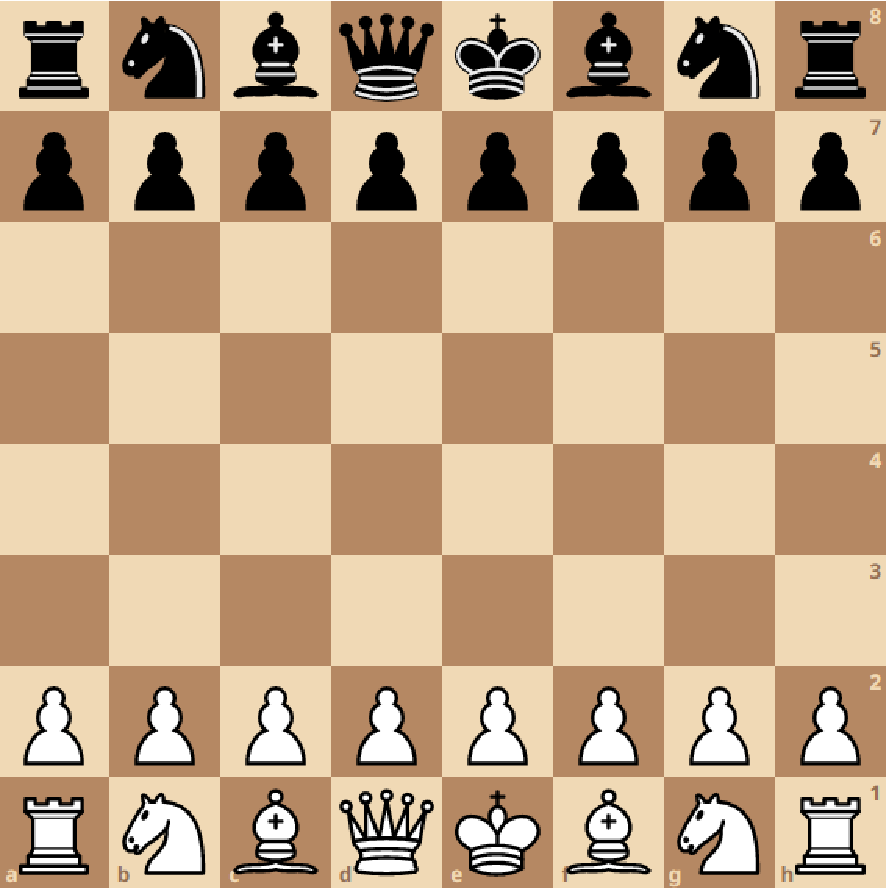
\includegraphics[width=10cm]{frontmatter/figure/scacchiera_iniziale.pdf}
    \centering
    \caption{Disposizione dei pezzi all'inizio della partita}
    \label{fig:checkmate}
\end{figure}
\subsection{Come si muovono i pezzi}
Ogni tipologia di pezzo segue delle regole ben precise nei movimenti. Non è possibile, ad esempio, muovere dei pezzi attraversando altri pezzi (eccetto per il cavallo, che può "saltarli") e ogni casella può essere occupata soltanto da un pezzo per volta. Negli scacchi è possibile liberare una casella dall'occupazione avversaria, \textbf{catturando} il pezzo interessato ed eliminandolo dalla scacchiera fino alla fine della partita. Come accennato in precedenza, ogni pezzo si muove in modo diverso dall'altro. In particolare:
\begin{itemize}
    \item il \textbf{re} può muoversi soltanto di una casella per volta nelle 8 direzioni disponibili (fig. \ref{fig:re}), ma non è possibile spostarlo in una casella che lo metterebbe sotto \textbf{scacco} (minacciato da un pezzo avversario);
    \item la \textbf{regina} può muoversi in qualsiasi direzione seguendo una linea retta sia in orizzontale che in diagonale di quante caselle vuole (fig. \ref{fig:regina}). Come tutti gli altri pezzi, in caso di cattura di un pezzo avversario il suo movimento si conclude nella casella precedentemente occupata dal pezzo catturato;
    \item la \textbf{torre} può muoversi di quante caselle si desidera, ma soltanto in avanti, indietro e di lato (fig. \ref{fig:torre}). Le due torri, quando ben collegate, si proteggono a vicenda e risultano estremamente utili;
    \item l'\textbf{alfiere} può muoversi in diagonale (fig. \ref{fig:alfiere}), e in virtù di questa caratteristica ogni alfiere rimane sullo stesso colore fino alla fine della partita (uno sulle caselle chiare e l'altro sulle caselle scure);
    \item il \textbf{cavallo} segue dei movimenti "a L" (fig. \ref{fig:cavallo}), avanzando di due caselle in una direzione e poi di un'altra casella a 90°;
    \item il \textbf{pedone} può muoversi di una sola casella in avanti (oppure anche due se è la sua prima mossa), ma cattura i pezzi avversari in diagonale di una casella (fig. \ref{fig:pedone}). Non è possibile indietreggiare, né catturare all'indietro. Inoltre, se un pedone raggiunge il lato opposto della scacchiera può trasformarsi in qualsiasi altro pezzo.
\end{itemize}
\newpage


\newpage

% Per affiancare due figure
\begin{figure}[!htb]
\begin{minipage}[b]{7cm}
\centering
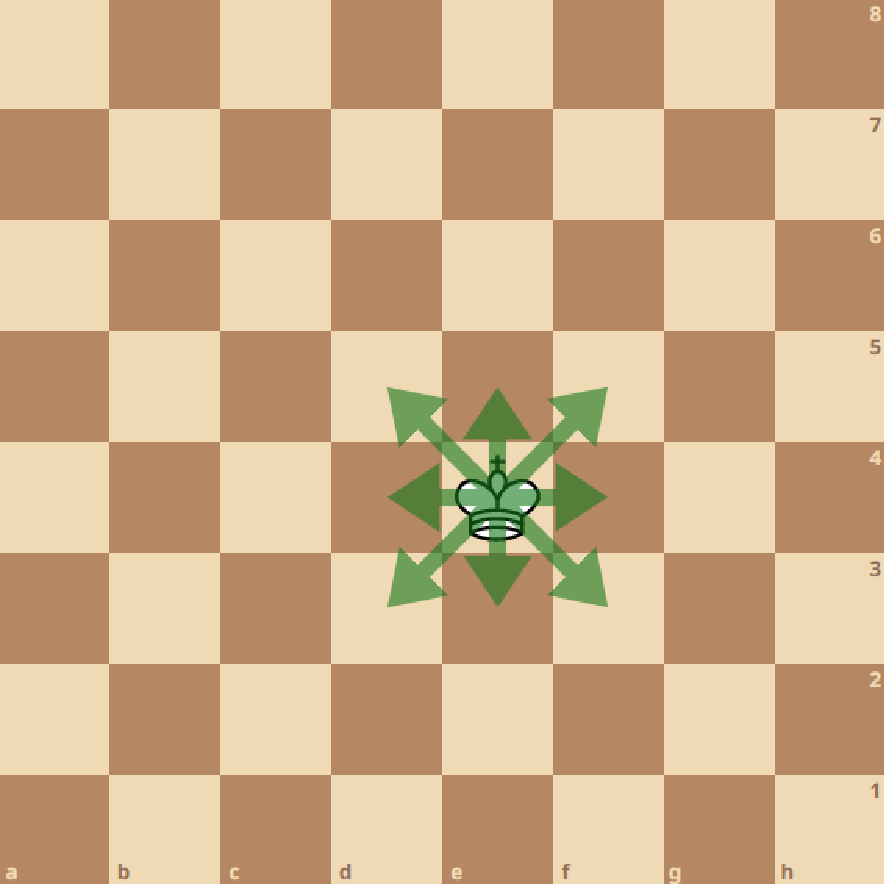
\includegraphics[width=6.3cm]{frontmatter/figure/movimento_re.pdf}
\caption{Movimenti del re}
\label{fig:re}
\end{minipage}
\hspace{1mm}
\begin{minipage}[b]{7cm}
\centering
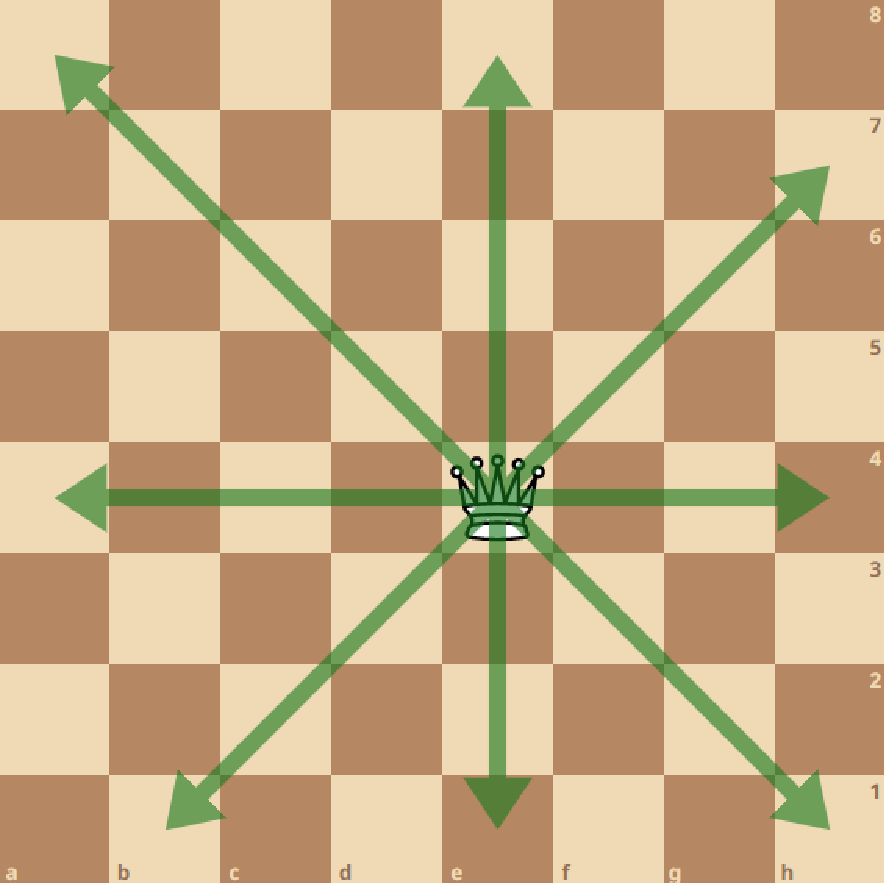
\includegraphics[width=6.3cm]{frontmatter/figure/movimento_regina.pdf}
\caption{Movimenti della regina}
\label{fig:regina}
\end{minipage}
\end{figure}

\begin{figure}[!htb]
\begin{minipage}[b]{7cm}
\centering
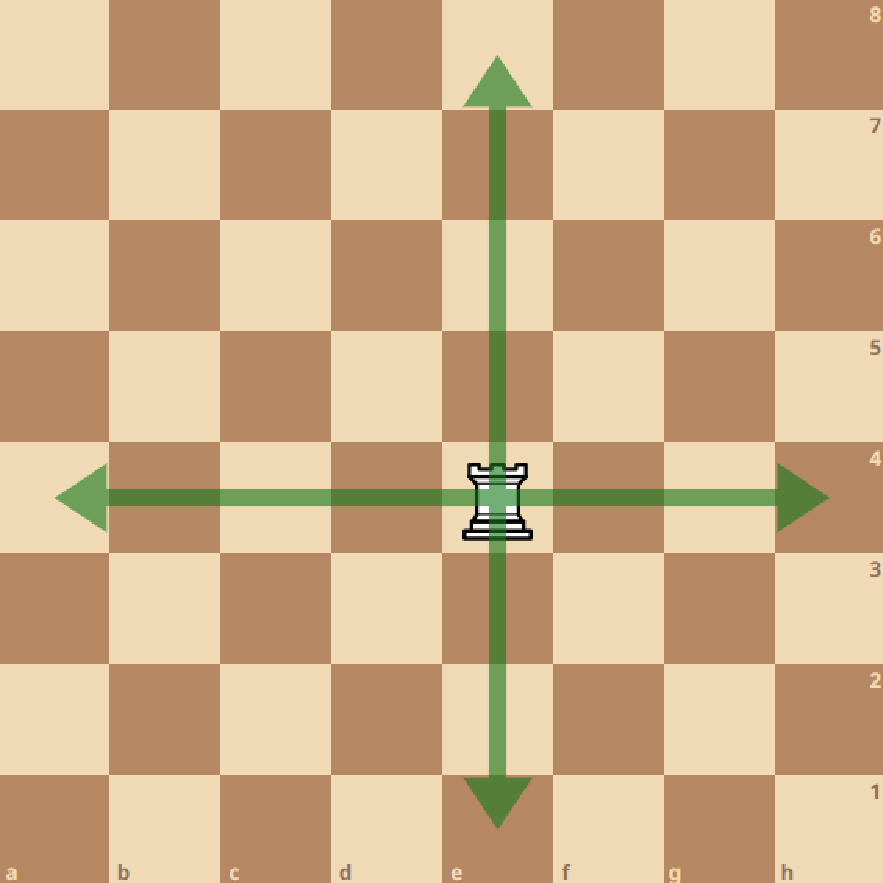
\includegraphics[width=6.3cm]{frontmatter/figure/movimento_torre.pdf}
\caption{Movimenti della torre}
\label{fig:torre}
\end{minipage}
\hspace{1mm}
\begin{minipage}[b]{7cm}
\centering
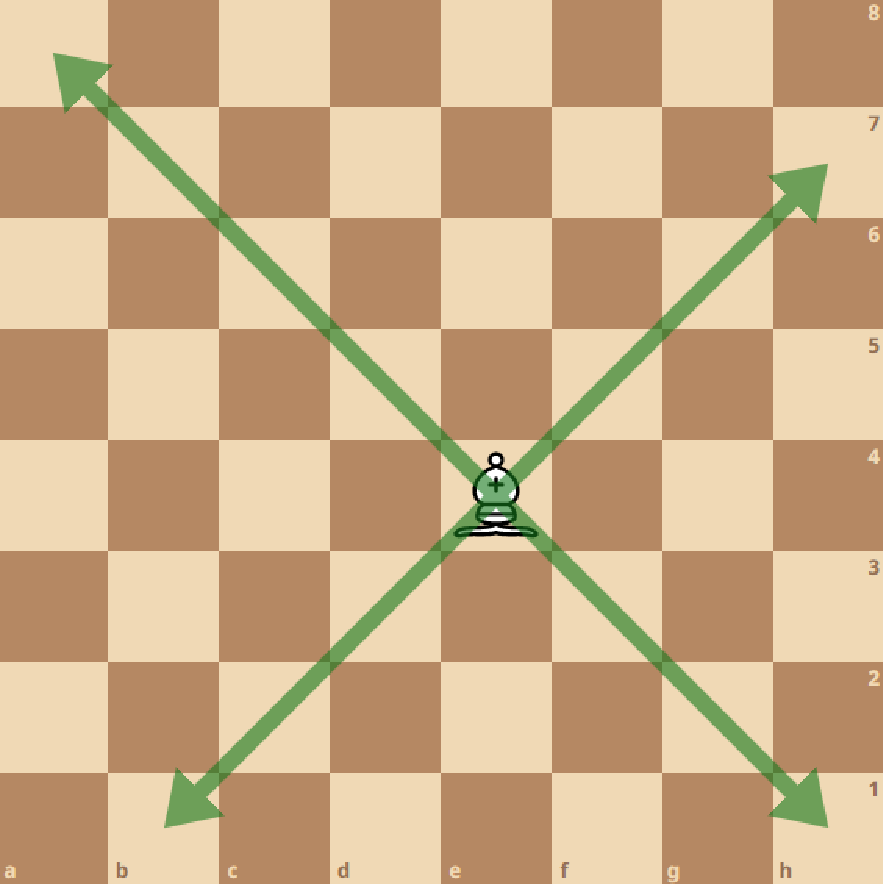
\includegraphics[width=6.3cm]{frontmatter/figure/movimento_alfiere.pdf}
\caption{Movimenti dell'alfiere}
\label{fig:alfiere}
\end{minipage}
\end{figure}

\begin{figure}[!htb]
\begin{minipage}[b]{7cm}
\centering
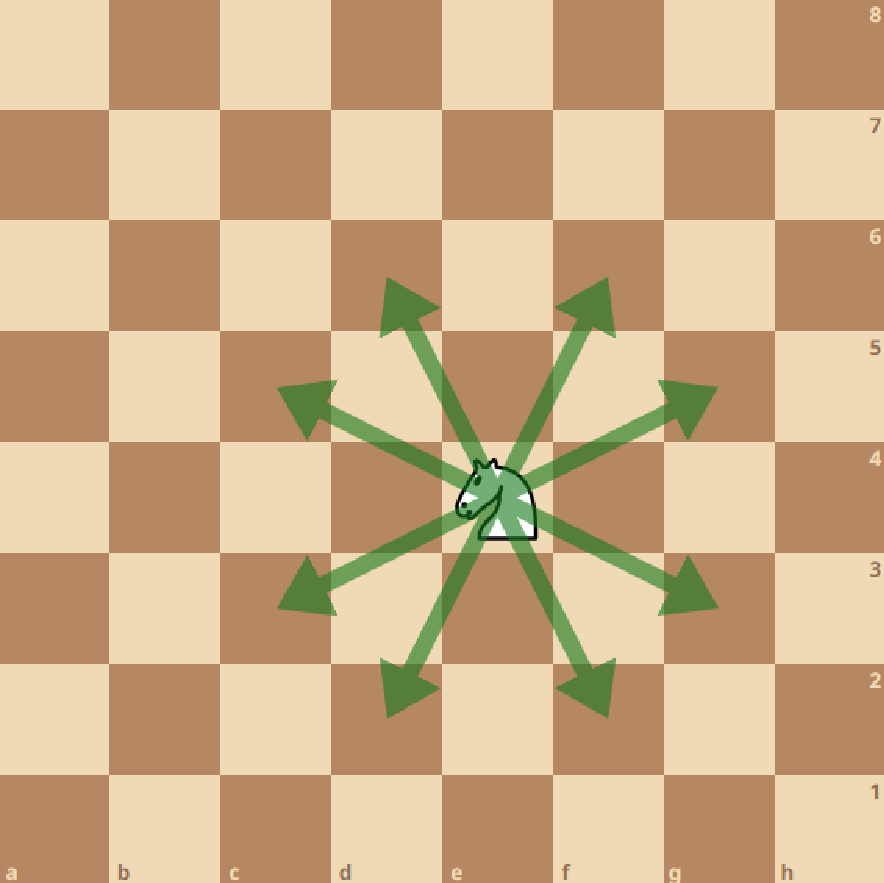
\includegraphics[width=6.3cm]{frontmatter/figure/movimento_cavallo.pdf}
\caption{Movimenti del cavallo}
\label{fig:cavallo}
\end{minipage}
\hspace{1mm}
\begin{minipage}[b]{7cm}
\centering
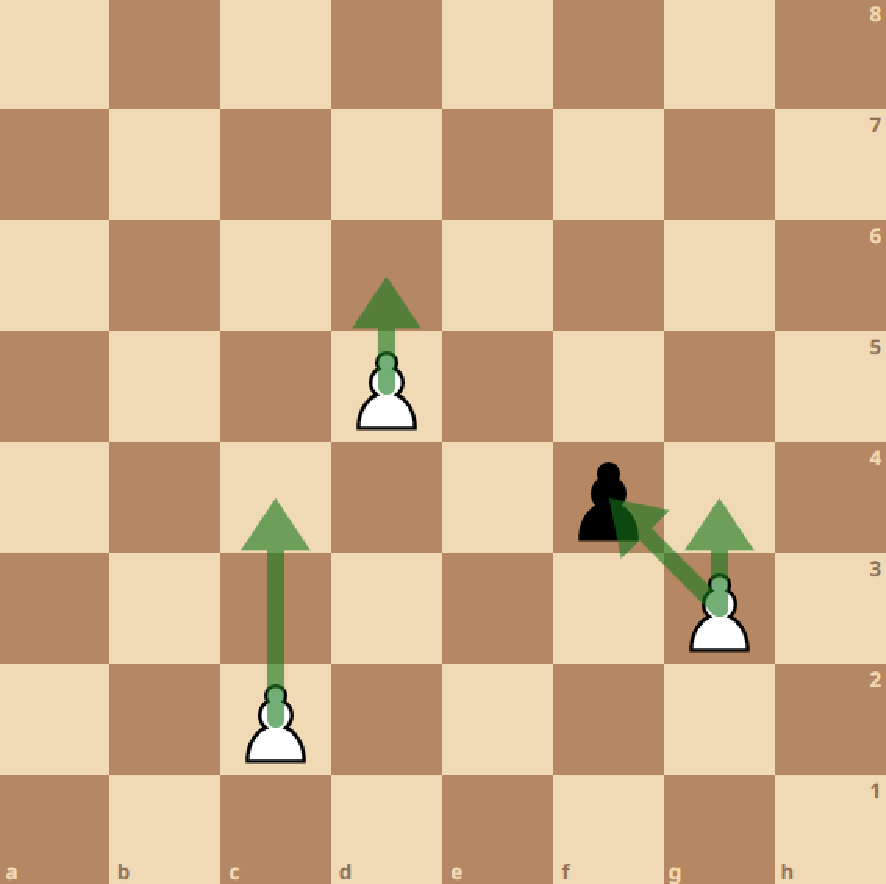
\includegraphics[width=6.3cm]{frontmatter/figure/movimento_pedone.pdf}
\caption{Movimenti del pedone}
\label{fig:pedone}
\end{minipage}
\end{figure}



Negli scacchi è possibile effettuare l'\textbf{arrocco}: si tratta di una mossa speciale che consente non solo di mettere il proprio re al sicuro, ma anche di sviluppare una torre portandola in gioco. Per effettuare l'arrocco si sposta il re di due caselle verso destra o sinistra e si sposta la torre di una casella accanto al re, ma in direzione opposta. Tuttavia, non è possibile effettuare l'arrocco se il re o la torre in questione siano già stati mossi in un turno precedente, o se le caselle interessate nell'arrocco siano occupate da altri pezzi o controllate da pezzi avversari. 
\begin{figure}[!htb]
    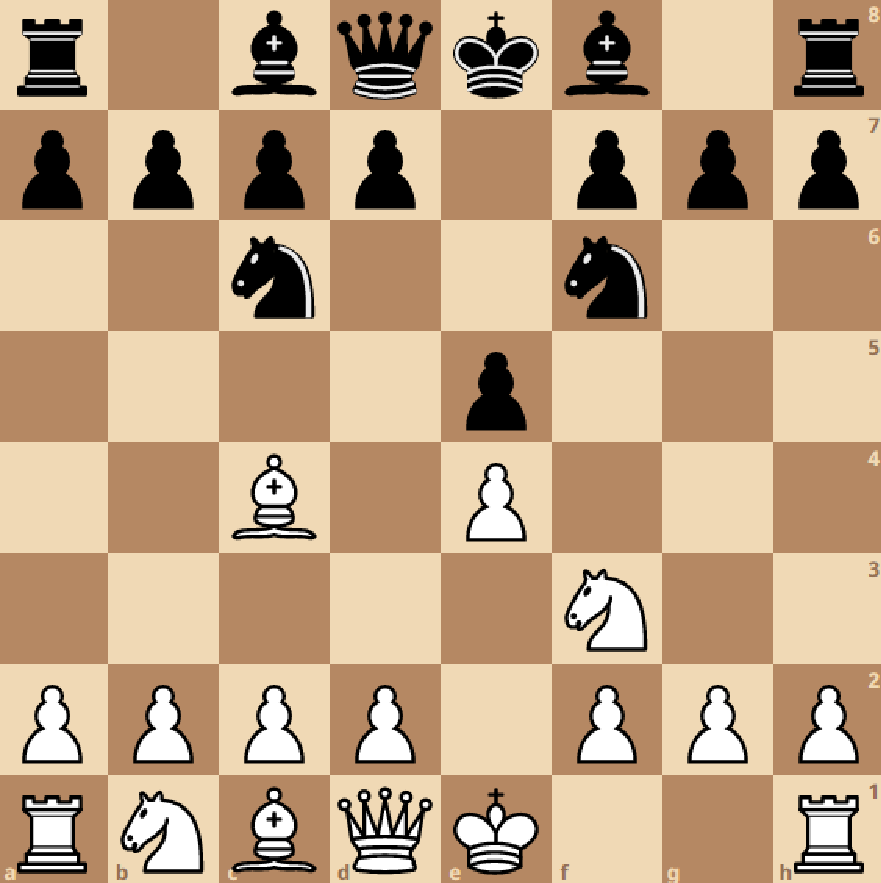
\includegraphics[width=8.4cm]{frontmatter/figure/arrocco_prima.pdf}
    \centering
    \caption{Preparazione all'arrocco}
    \label{fig:checkmate}
\end{figure}
\begin{figure}[!htb]
    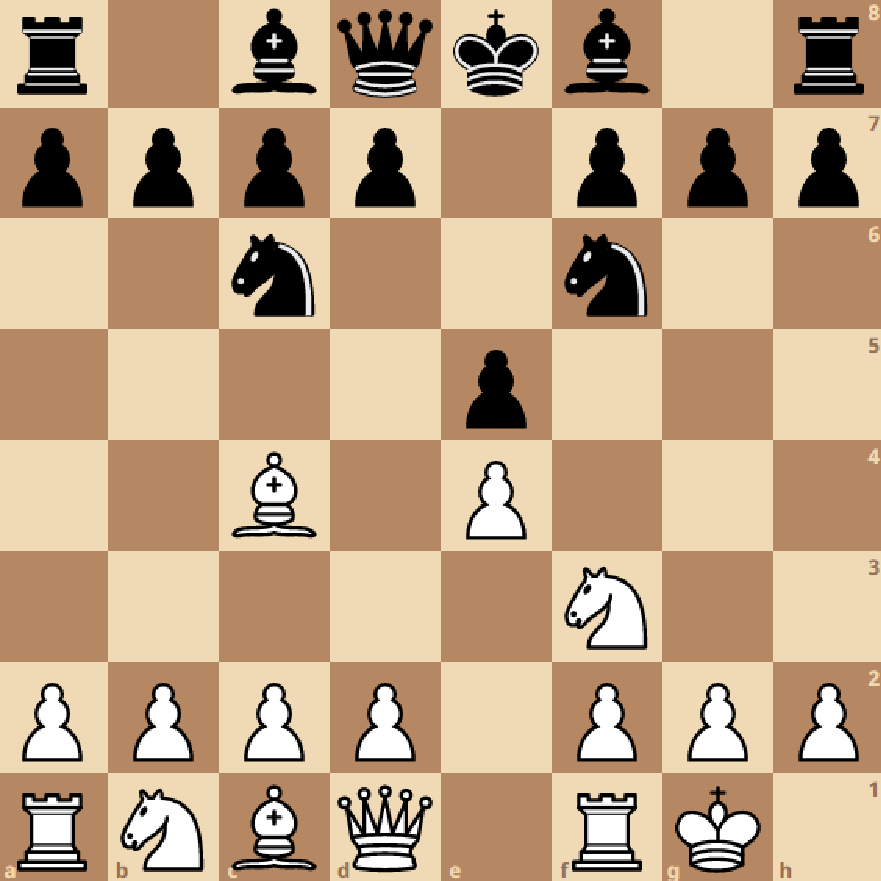
\includegraphics[width=8.4cm]{frontmatter/figure/arrocco_dopo.pdf}
    \centering
    \caption{Posizione dopo l'arrocco}
    \label{fig:checkmate}
\end{figure}
\newpage
Un'altra regola speciale degli scacchi riguarda la cattura \textbf{en passant} dei pedoni: se un pedone muove di due caselle alla sua prima mossa portandosi accanto a un pedone avversario (saltando la casella su cui sarebbe stato catturato), l'avversario ha la possibilità di catturare quel pedone occupando la casella aventi in diagonale. Questa speciale cattura deve però essere effettuata nel turno immediatamente successivo all'avanzamento del pedone, altrimenti non sarà più possibile farlo.
\begin{figure}[!htb]
    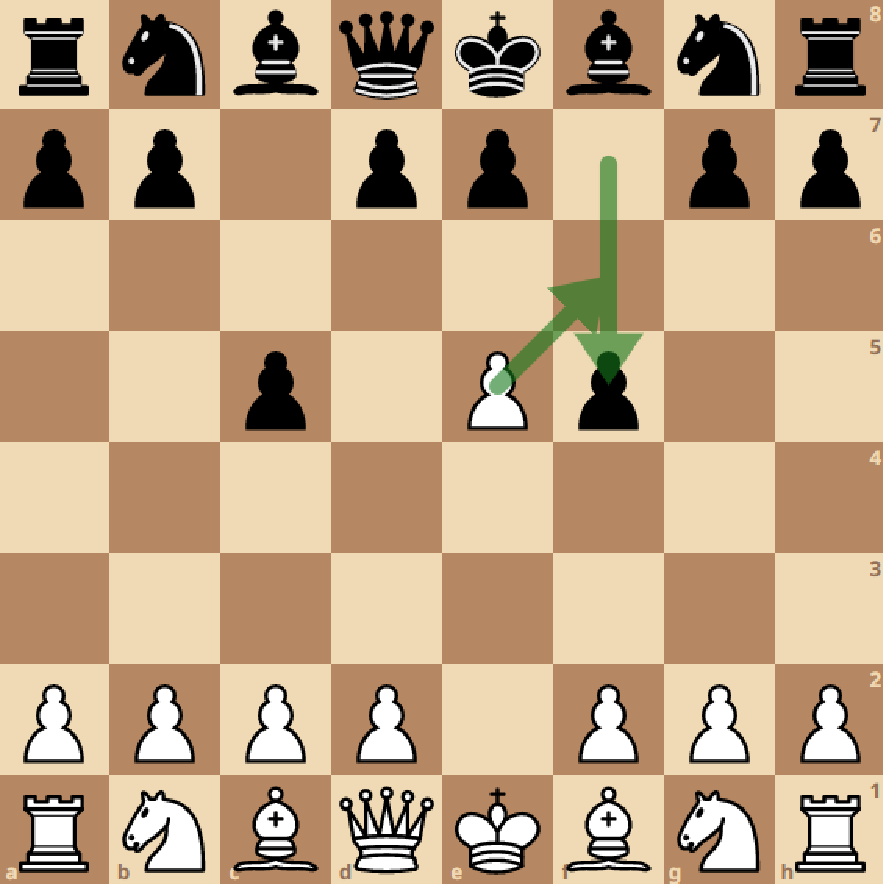
\includegraphics[width=8.4cm]{frontmatter/figure/enpassant_prima.pdf}
    \centering
    \caption{Posizione prima della cattura en passant}
    \label{fig:checkmate}
\end{figure}
\begin{figure}[!htb]
    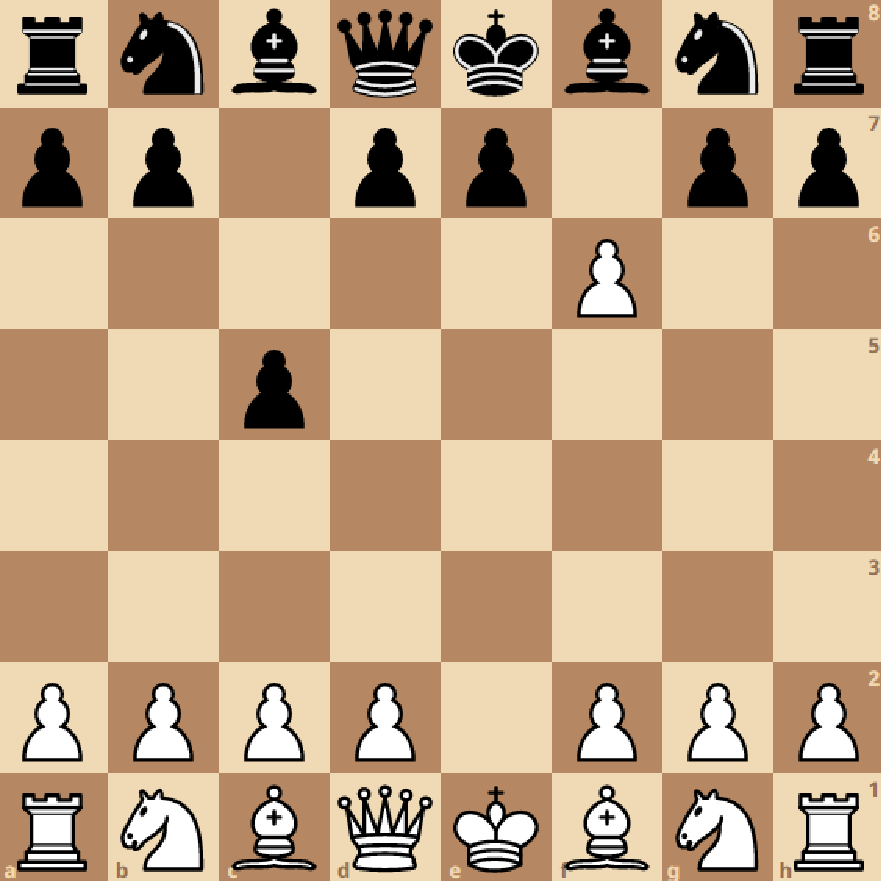
\includegraphics[width=8.4cm]{frontmatter/figure/enpassant_dopo.pdf}
    \centering
    \caption{Cattura en passant}
    \label{fig:checkmate}
\end{figure}
\newpage
Nel gioco degli scacchi, è \textbf{sempre} il giocatore con i pezzi bianchi a muovere per primo. Questo privilegio porta un leggero vantaggio al bianco, che nella maggior parte dei casi imposterà piani d'attacco e di difesa già dalla prima mossa.

\subsection{Vincere una partita a scacchi}
\label{cap: valore_pezzi}
L'obiettivo del gioco degli scacchi è quello di attaccare il re avversario, cercando di impedirgli di sottrarsi alla minaccia. Esistono, infatti, tre modi per difendere il proprio re da uno scacco: spostandolo in una casella libera e non minacciata, interponendo un proprio pezzo oppure catturando il pezzo che minaccia il re. Se il re non può liberarsi dallo scacco in nessuno dei tre modi, la partita viene dichiarata finita per \textbf{scacco matto}. Esistono casi in cui una partita di scacchi si conclude con una \textbf{patta}, cioè in parità, senza vincitori. Ciò accade principalmente per 5 motivi:
\begin{itemize}
    \item tutti i propri pezzi sono stati catturati, tranne il re. Non è possibile eseguire alcuna mossa legale, ma contemporaneamente il re non è sotto scacco. In questo caso, la partita finisce per \textbf{stallo}:
    \item i giocatori possono semplicemente accordarsi e smettere di giocare;
    \item non è possibile dare scacco matto in alcun modo (per esempio, un re e un alfiere contro un re);
    \item è stata ripetuta la stessa posizione per la terza volta nel corso della partita;
    \item sono state giocate 50 mosse consecutive senza catturare alcun pezzo.
\end{itemize}
Cercare di proteggere i propri pezzi è uno dei punti chiave per vincere la partita. Di solito i giocatori di scacchi assegnano a ciascun pezzo un numero che ne indichi il valore, in modo da portare avanti delle strategie vincenti. Il \textbf{re} ha il valore più alto, poiché la sua perdita causerebbe la sconfitta. La \textbf{regina} vale 9 punti, essendo il pezzo più importante dopo il re data la sua elevata libertà di movimento che potrebbe causare problemi all'avversario. Una \textbf{torre} vanta ben 5 punti, e due torri usate in sinergia sarebbero più potenti di un'unica regina. All'\textbf{alfiere} e al \textbf{cavallo} vengono assegnati valori pressoché simili, intorno ai 3 punti. Il \textbf{pedone} vale 1 punto. Sebbene esistano dei valori convenzionali comunemente assegnati, è bene tenere a mente che il valore corretto di ciascun pezzo dipende in realtà dalle sue capacità considerate in precisi momenti di una partita in corso\cite{itwiki:106074354}. 

\section{Struttura della tesi}
La trattazione del lavoro di tesi è strutturata secondo il seguente elenco:
\begin{itemize}
    \item \textbf{Introduzione}: viene fornita una panoramica dello studio effettuato, con particolare attenzione alle motivazioni, 
    agli obiettivi e ai risultati del lavoro svolto;
    \item \textbf{Ruolo del gioco degli scacchi nell'Intelligenza Artificiale}: l'attenzione viene spostata sulla storia che ha portato il gioco degli scacchi ad essere trattato con le tecniche moderne e sull'analisi di alcune delle tecnologie attualmente in uso;
    \item \textbf{Progettazione e implementazione}: si esaminano nel dettaglio la progettazione e l'implementazione del lavoro svolto;
    \item \textbf{Conclusioni e sviluppi futuri}: vengono presentate riflessioni e considerazioni di carattere generale con eventuali riferimenti agli sviluppi futuri.
\end{itemize}
